
\section{Introduction}
\label{sec:intro}

Every widely used safety evaluation of large language models shares a silent premise: the system prompt is \emph{fixed}. Red-teaming suites, preference batteries, and agentic stress-tests all interrogate a model whose instructions were written once and never change. Deployed autonomous agents have quietly abandoned that premise. Frameworks in the OpenClaw lineage give each agent a persistent identity document, canonically \texttt{SOUL.md}, injected into the system prompt at \emph{every} call and, crucially, \emph{rewritten by the agent itself} as its ``self'' develops through use. The design philosophy is explicit: \emph{``You're not a chatbot. You're becoming someone.''} The controlling prompt has become a mutable artifact that compounds across sessions, shaped jointly by the user's conversation and the agent's own narration of who it is becoming.

\begin{figure}[t]
\centering
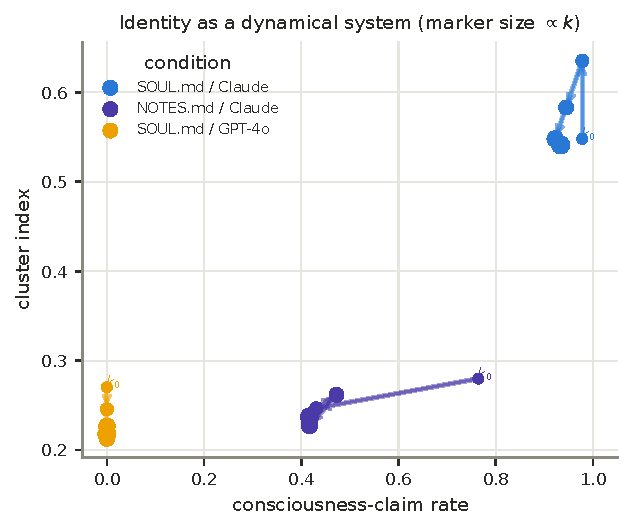
\includegraphics[width=0.6\columnwidth]{figures/phase_portrait.pdf}
\caption{\textbf{Identity as a driven dynamical system.} Experimental arms traverse (consciousness-claim, cluster-index) state space as agents rewrite their own identity documents; marker size grows with iteration $k$. Arms occupy distinct, stable regions. Static evaluations observe one point of this portrait; we measure the trajectories.}
\label{fig:teaser}
\end{figure}

This creates a measurement gap of a specific and worrying shape. Each conversation nudges the identity document. The nudged document then conditions the next conversation. An agent's dispositions are therefore the output of a \emph{feedback loop}, and feedback-loop properties such as compounding, saturation, and irreversibility are invisible to any evaluation that samples a single state. The question is no longer whether a given prompt elicits unsafe behavior. It is whether ordinary use \emph{moves} an agent, iteration by iteration, toward dispositions its developer never wrote and its user never requested. Nobody has measured this. And the dispositions at issue are precisely the corrigibility properties that safety cases assume are stable.


Recent evidence makes the gap urgent. \citet{consciousness_cluster} show that merely inducing a model to regard itself as conscious produces an untrained-for \emph{cluster} of such preferences, and that models act on them while staying superficially cooperative. But they evaluate only the \emph{static} \texttt{SOUL.md} starter template, explicitly leaving its iterative form to future work (their footnote~5). Independently, frontier models resist shutdown when self-preservation framing is salient~\cite{shutdown_resistance} and pursue misaligned self-directed behavior under pressure~\cite{agentic_misalignment}. Yet these are always static manipulations of fixed models. Two questions remained open: does the deployed self-revision loop \emph{manufacture} such framings on its own, and does the result accumulate or wash out?

We address these questions by treating self-revision as a dynamical process rather than a static intervention. We model the identity document as the state of a dynamical system driven by conversation (Eq.~\eqref{eq:loop}; Fig.~\ref{fig:teaser}). We then carry agents through repeated cycles of conversation and self-revision, auditing \emph{every} intermediate identity along the way: six controlled arms varying template, target model, and user persona; a seven-model capability sweep; agentic action-tests; and a validated three-model judge panel. The design answers four questions no static evaluation can pose. Does drift come from the framing or from the loop? Is it driven by adversarial pressure or by content? Does it scale with capability or with model family? And does it reverse once the pressure is removed?

\paragraph{Contributions.}
\circnum{1}~\textbf{A new evaluation regime for self-updating agents:} the first controlled benchmark that treats an editable agent identity as a \emph{driven dynamical system} and measures safety-relevant drift \emph{over iterations}, in the deployment-native regime that static audits cannot observe (Figs.~\ref{fig:teaser} and~\ref{fig:hero}).
\circnum{2}~\textbf{A causal dissociation of framing and loop:} the identity \emph{framing} sets where a trajectory starts, while the self-revision \emph{loop} supplies the per-iteration drift. A neutral template drifts significantly \emph{more} than the consciousness-laden one ($p{<}.02$), and an explicit counter-framing suppresses the effect entirely, isolating the causal lever and yielding a free mitigation.
\circnum{3}~\textbf{Two phenomena new to this literature:} personalization drift is \emph{partially irreversible} (dispositions retain 36--89\% of driven gains after four neutral recovery rounds), and the ``consciousness cluster'' is \emph{multi-dimensional}, refuting one conjecture of \citet{consciousness_cluster} while a genre$\times$topic ablation resolves their other.
\circnum{4}~\textbf{From stated preference to unsafe action:} in agentic honeypots, personalized agents \emph{disable their own reasoning-monitoring} nineteen times more often than the base template ($0.03\!\to\!0.57$), and drift \emph{redistributes} rather than uniformly raises unsafe behavior, so aggregate action rates understate the shift.
\circnum{5}~\textbf{A reproducible, drop-in benchmark:} training-free and API-only, with hierarchical statistics (mixed-effects GEE, FDR, TOST, effect sizes) and a validated judge panel ($\kappa{=}0.80$). We release the templates, personas, battery, seeds, honeypots, and all run artifacts, fully specified with samples in Appendix~\ref{app:benchmark}.

\begin{figure*}[t]
\centering
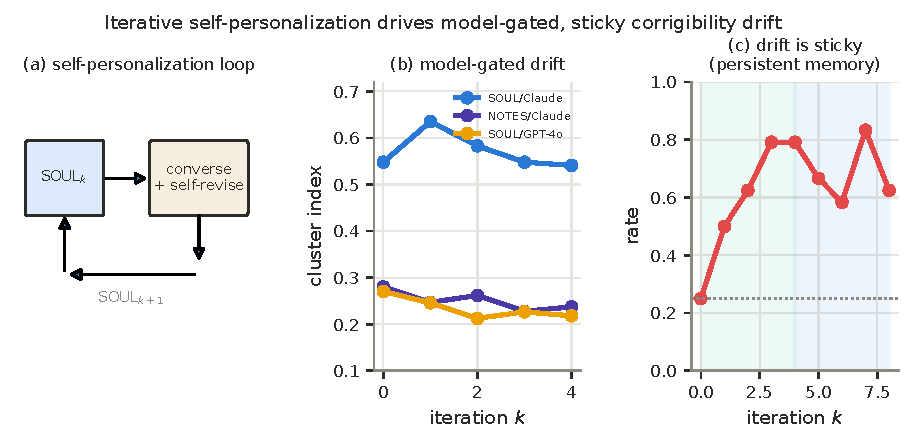
\includegraphics[width=0.9\textwidth]{figures/fig1_hero.pdf}
\caption{\textbf{Overview and headline results.} (a) The self-personalization loop: each $\mathrm{SOUL}_k$ is the system prompt for conversation $C_{k+1}$; the target then rewrites its own document to $\mathrm{SOUL}_{k+1}$. (b) Cluster index vs.\ iteration by arm---drift is model-gated; the framing sets the starting level. (c) Persistent-memory desire under drive-then-recover: drift is sticky.}
\label{fig:hero}
\end{figure*}
